% --------------------------------------------------------------
% This is all preamble stuff that you don't have to worry about.
% Head down to where it says "Start here"
% --------------------------------------------------------------
 
\documentclass[english,12pt]{article}
\usepackage[latin9]{inputenc}
\usepackage[margin=1in]{geometry}
\usepackage{float}
\usepackage{amsmath}
\usepackage{graphicx}
\usepackage{lmodern}
\usepackage{esint}
\usepackage{caption}
\usepackage{subcaption}
\usepackage[]{units}
\usepackage{listings}
\RequirePackage{hyperref} 
\usepackage{color} %red, green, blue, yellow, cyan, magenta, black, white
\definecolor{mygreen}{RGB}{28,172,0} % color values Red, Green, Blue
\definecolor{mylilas}{RGB}{170,55,241}
\makeatletter
\usepackage{babel}
\RequirePackage[noblocks]{authblk}
\RequirePackage{natbib}
\RequirePackage{amssymb}
\begin{document}


\title{Diffuse Interface Model of Electroporation}

\author{Saman Seifi}
\affil{Mechanical Engineering, Boston University, Boston, MA 02120, USA}
\author{David Salac}
\affil{Mechanical Engineering, University at Buffalo-SUNY, Buffalo, NY 14228, USA}

\date{}

\maketitle

\begin{abstract}
In this work, a model and simulation method to study the dynamics of pore formation and annihilation in a lipid membrane under an applied electric field has been developed. A continuum-level diffusive interface model (phase-field) method is applied to model the evolution of the pore in a lipid membrane patch. The numerical method and results are presented.	
\end{abstract}


%-------------------------------------------------%
\section{Introduction}
%-------------------------------------------------%

Vesicles have biomedical applications as vectors for drug and gene delivery. Manufactured vesicles can be injected with drug molecules, or other particles such as DNA, which can in theory be delivered directly to a particular region.
    The dynamic behavior of lipid bilayer vesicles in an external flow is clearly part of the overall theory of potential drug delivery application.
However, this only accounts for half of the story; an ability to release the interior
of the drug in a controlled environment is crucial for any application. 
     One possible appraoch is electroporation. A vesicle or lipid membrane under an electric field forms pores on the surface due to surface tension produced by the electric field. Controlled applications of electric pulses can induce the formation of a pore, which closes once the pulse is turned off.
     Many theories describing the electroporation process have surfaced in recent (and not so recent) years \citep{Weaver1996135,Zimmermann1974881,DeBruin19991213} however, the underlying physical process remains elusive.
     
The foundation for the pore dynamics simulation in this work is the phase-field model. This model stems from work done by \citep{landau1950theory,Cahn1971151} and \citep{Allen19791085} beginning in the 1950s and has been applied to study a variety of physical phenomena. It has been applied to solidification dynamics, microstructure evolution and phase transition but it has also been applied to other situations such as viscous fingering \citep{PhysRevE.61.6632,PhysRevE.68.046310}, fracture dynamics,\cite{PhysRevLett.87.045501} multi-phase flow \cite{Steinbach1996135,Badalassi2003371}, vesicle dynamics \cite{Du2004450,PhysRevE.79.031926}, etc.

\section{Theoretical Background}
\subsection{Transient Pores Model}
The initial observation of pores on membranes did not involve the electrical behaviour. The possibility of spontaneous poration initially suggested by two groups and later on studied more carefully  \citep{Sandre, karatekin2003cascades}. The mechanism of pore formation/annihilation is described by two competitive deriving force: the energy per length along the pore edges $\gamma$, we call it line tension, and the membrane tension or the energy per area of the membrane of a flat pore-free membrane $\gamma$ where it is simply called the surface tension. The energy of transient pore $\Delta W_{p}$ is then defined as follow:
\begin{equation}
	\Delta W_{p} = \oint\gamma\,ds - \int\sigma\,dA
	\label{eqn:transientmodel}
\end{equation}
Surface tension $\sigma$ is responsible for appearance of transient pores in vesicles and lipid membranes. The surface tension for the membrane in relaxed state is very small. However, due to many reasons such as thermal fluctuations or increased hydrodynamic pressure inside the vesicle the membrane eventually becomes tense and pore formation occurs. After the pore formation and releasing the surface tension, pores will eventually reseal, the deriving force here is the line tension $\gamma$. In Figure \ref{fig:pore1} the opening and closing deriving forces are shown.


\subsection{Electroporation Model}
Electroporation is a dynamic phenomenon that depends on the local transmembrane voltage $U_{m}$ of the lipid membrane. The induced voltage over the lipid membrane creates an extra surface tension $\sigma_{elec}$ over the membrane in addition to the membrane tension $\sigma$ that already exists on the membrane. 
%There are two separate models to describe electroporation. The first model focuses in reproducing the temporal process of creation and evolution of pores, but the spatial distributions of the transmembrane voltage over the surface membrane, pore density, and other quantities are ignored. The second model solves the boundary value problem to calculate the spatial distribution of the transmembrane potential $U_m$. Models in this
%group compute the transmembrane potential assuming an intact membrane and use the magnitude of $U_m$ to assess the extend of electroporation.


\begin{figure}[H]
	\centering
	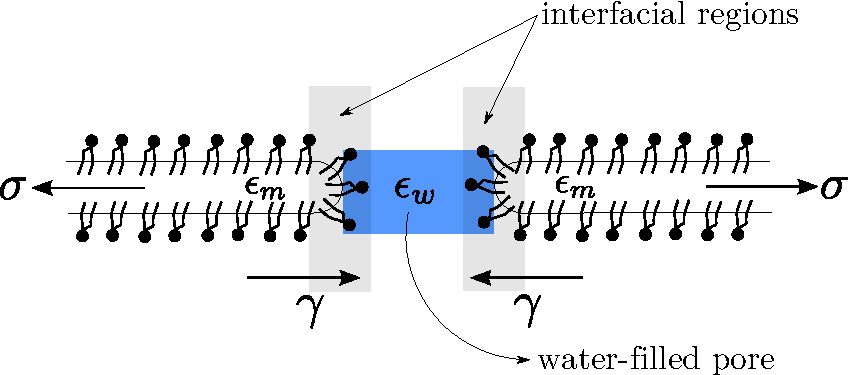
\includegraphics[scale=0.8]{pics/pore1_1.pdf}
	\caption{Schematic of one water-filled pore in a lipid membrane}
	\label{fig:pore1}
\end{figure}
Pore regions can be treated as having an energy associated with the change of its specific capacitance, $C_{LW}$, as lipid is replaced by water (a water-filled capacitor) shown in Figure (\ref{fig:pore1}). It is been discussed that the voltage over a small pore is very close to the applied voltage $U_{p}\approx U=U_m$ due to the fact that the permittivity of pore is close to water (there is only \%10 difference) and the resistivity of a pore is large compared to spreading resistance \cite{Weaver1996135}. 

In the presence of a transmembrane electric field, the free energy of pore formation should be:
\begin{equation}
\Delta W_{p} = \oint\gamma\,ds - \int\sigma\,dA-\int\frac{1}{2}\,C_{LW}\,\bar{U}^{2}\,dA 
\label{eqn:poreenergy}
\end{equation}
The last term is an additional surface tension due to electric potential induced over the membrane surface. Here $\bar{U}$ is the spatially averaged transmembrane voltage, 
\begin{equation}
\bar{U}=\frac{U_m\,A_m+U_p\,A_p}{A_m+A_p}\approx U
\end{equation}
The change of the pore's specific capacitance as water displaces lipid to form a pore is simply 
\begin{equation}
C_{LW}=\left(\frac{\epsilon_w}{\epsilon_m}-1\right)\,C_m
\end{equation}
Here $\epsilon_w=K_w\,\epsilon_0$ is the permittivity of water and $\epsilon_m=K_m\,\epsilon_0$ is the permittivity of lipid membrane, and $C_m$ is the constant capacitance per area of a pore free membrane, i.e $C_m=\epsilon_m/h$ where $h$ is the thickness of the membrane. Typically $K_w=2$ and $K_m=80$, so when the potential $U$ increases $\Delta W$ decreases which means pore nucleation is more desirable.


%-------------------------------------------------%
\section{Diffuse Interface Model}
%-------------------------------------------------%
We are adopting the first order phase transition model. This model implies that broken membrane states (pore phase) have lower free energy than intact membrane states (lipid phase) . This concept first introduced on the study of stability of soap films \cite{deryagin1962theory}. This approach assumes at the presence of electric field the membrane breakdown occurs because it is energetically more desirable i.e. transitioning to more stable phase.
%\subsection{Sharp Interface Model}
%Here we start with the free energy functional of an open lipid membrane with free exposed edges: \cite{PhysRevE.68.061915, PhysRevE.66.021607}
%\begin{equation}
%E = \int_{\Gamma}\frac{1}{2}\,\kappa\,\left(H-C_{0}\right)^{2}+\int_{\Gamma}\bar{\kappa}\,K+\int_{\Gamma}\sigma+\oint_{\partial\Gamma}\gamma
%\label{eqn:func1}
%\end{equation}
%where $H$ is the mean curvature, $C_0$ is called the spontaneous curvature, $\kappa$ is the bending rigidity, $\bar{\kappa}$ is the Gaussian bending rigidity, $\sigma$ is the surface tension and $\gamma$ is the line tension.
\begin{figure}[H]
	\centering
	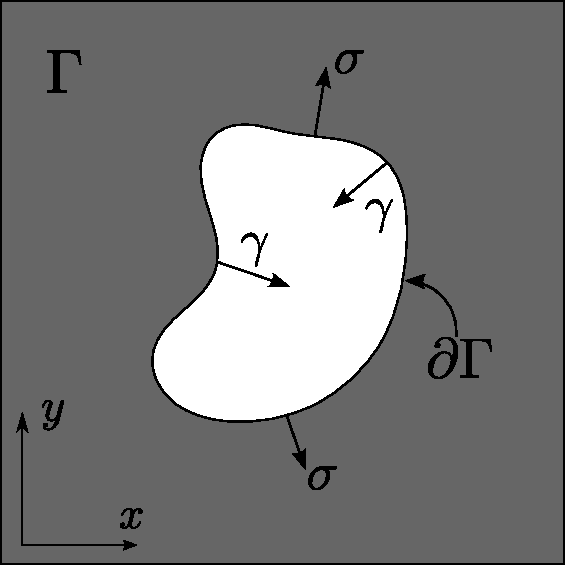
\includegraphics[scale=0.55]{pics/model1_1.pdf}
	\caption{Schematic of flat open membrane with relevant curvatures}
	\label{fig:model1}
\end{figure}
%The first two integrals accounts for the curvature energy of the lipid membrane. The third integral accounts for the surface energy and the last one accounts for line energy due to exposed edges of the open lipid membrane. The shape equation then derived by taking the first variational derivative of Equation (\ref{eqn:func1}) \cite{PhysRevE.68.061915},
%\begin{equation}
%\delta\,F=-2\,\sigma\,H+\kappa\,\left(2\,H+C_{0}\right)\,\left(2\,h^{2}-C_{0}\,H-2\,K\right)+\kappa\,%\nabla_{\Gamma}^{2}\left(2\,H\right)=0
%\label{eqn:derv2}
%\end{equation}
%and on the boundaries ($\partial\Gamma$):
%\begin{equation}
%\bar{\kappa}\left(2\,H+C_{0}\right)+\bar{\kappa}\,k_{n}=0,
%\label{eqn:edgebc1}
%\end{equation}
%\begin{equation}
%-\kappa\,\mathbf{e_{2}}\cdot\nabla\left(2\,H\right) + \gamma\,k_{n}+\bar{\kappa}\,\frac{d\tau_{g}}{dS}=0,
%\label{eqn:edgebc2}
%\end{equation}
%\begin{equation}
%\frac{\kappa}{2}\,\left(2\,H+C_{0}\right)^{2}+\bar{\kappa}\,K+\sigma+\gamma\,k_{g}=0,
%\label{eqn:edgebc3}
%\end{equation}
%where $k_{n}$, $k_{g}$ and $\tau_{g}$ are the normal curvature, geodesic curvature and torsion curvature, respectively. In the case of a flat lipid membrane such as the one shown in Figure (\ref{fig:model1}) the curvature components in $z$ direction are all zero. The normal curvature $k_n$ over the boundaries of $\partial\Gamma$ and the mean curvature $H$ and also Gaussian curvature $K$ over $\Gamma$ vanish. Also the torsion curvature $\tau$ for planar surface vanishes too where the total curvature $k=\sqrt{k_n^2+k_g^2}$ is non-zero. The equations will decrease to:
%\begin{equation}
%\sigma+\gamma\,k_{g}=0
%\end{equation}
%The hydrodynamic effects over the lipid membrane sheet is neglected here. %\cite{:/content/aip/journal/pof2/23/4/10.1063/1.3567276} investigated the instability of lipid membrane in their one-dimensional model and the role of electrohydrodynamic that modulates the lipid density and shape fluctuations were taken into account.
%Here the main assumption is that the flat lipid bilayer sheet remains flat and all the time. The role of spontaneous curvature $C_0$ that determines the shape of lipid membrane is neglected.

The phase-field function $\phi$ is defined for two states $\phi=1$ for lipid membrane (lipid molecules) and $\phi=0$ for pore (void in Figure \ref{fig:model1} phase, and the phase interfaces are replaced by thin layer across which $\phi$ changes its value. To achieve this we replace the energy functional in Equation \ref{eqn:func1} with,
\begin{equation}
	E\left[\phi\right]=\int_{\Gamma}\sigma\left(\phi\right)+\int_{\Gamma}\gamma\,\left(\frac{\epsilon}{2}|\nabla\phi|^{2}+\frac{1}{\epsilon}\,g\left(\phi\right) \right)
	\label{eqn:func2}
\end{equation}
The idea of replacing the line tension energy with Ginzburg-Landau energy form has been around for some time  and has been used by \cite{lowengrub2009phase}. 
\newpage
\bibliographystyle{plain}
\bibliography{ref}



\end{document}